\begin{problem}
  A small Lambertian source $\d A$ is centered at $P$
  and emits radiance $L$. The orientation of this patch is the same
  as that of a plane containing two points, $X_1$ and $X_2$.
  The point $X_1$ is the point on this plane that is closest to $P$,
  and the distance from $P$ to $X_1$ is $D$ as shown.
  \begin{figure}[H]
    \centering
    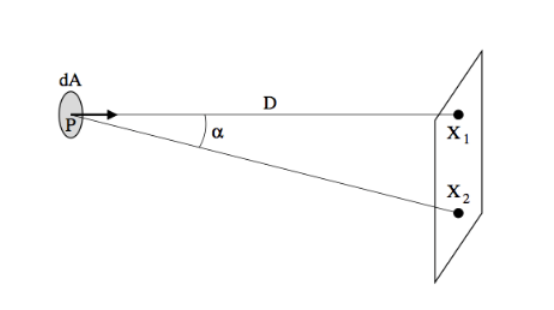
\includegraphics[width=0.5\textwidth]{figures/lambertian.png}
    \label{fig:1}
  \end{figure}
  \begin{enumroman}
    \newpage
    \item Calculate the solid angle subtended by $\d A$ at points $X_1$ and $X_2$.
      \begin{answer}
        The solid angle subtended by an area $\d A$ at a point $\bx$ that is a distance
        $r$ from $\d A$ is given by
        \[ \d\omega = \frac{\d A \cos\theta}{r^2}, \]
        where $\theta$ is the angle between the normal to $\d A$
        and the line from $\bx$ to $\d A$.
        In this case;
        \begin{enumarabic}
          \item Since $\d A$ has the same orientation as the plane containing $X_1$ and $X_2$,
            and we are given that $X_1$ is the point on this plane that is closest to $P$,
            then the normal at $\d A$ passes through $P$.
            Therefore, $\theta = 0$ and $\cos\theta = 1$.
            Therefore, $\displaystyle \d \omega_{X_1} = \frac{\d A}{D^2}$.~\label{item:1.1}
          \item As established in part~\ref{item:1.1}, the normal at $\d A$ passes through $P$.
            Therefore, the angle between the normal to $\d A$ and the line from $X_2$ to $\d A$
            is $\alpha$ as shown in the image.
            Let $D_2 = \norm{X_2 - P}$; then:
            \begin{align*}
              \cos\alpha &= \frac{D}{D_2} \\
              &\blue{\implies D_2 = \frac{D}{\cos\alpha}}.
            \end{align*}
            Therefore;
            \begin{align*}
              \d \omega_{X_2} &= \frac{\d A \cos\alpha}{D_2^2} \\
              &= \frac{\d A \cos\alpha}{D^2/\cos^2\alpha} \\
              &= \frac{\d A \cos^3\alpha}{D^2}.
            \end{align*}
            ~\label{item:1.2}
        \end{enumarabic}
      \end{answer}
    \newpage
    \item Calculate the irradiance $E$ incident on the plane at points
      $X_1$ and $X_2$, and calculate the ratio $E(X_1)/E(X_2)$.
      \begin{answer}
        The irradiance $E$ incident at a point $\bx$ is given by
        \[
          E(\bx) = \int_{H^2} L(\bx, \omega) \cos\theta \d\omega.
        \]
        To find the irradiance at single points $X_1$ and $X_2$,
        we do not have to integrate over the entire hemisphere
        but simply calculate
        \[
          E(\bx) = L \cos\theta \d \omega
        \]
        at the two points:
        \begin{enumarabic}
          \item The irradiance $E(X_1)$ incident on $X_1$ is given by
            \begin{align*}
              E(X_1) &= L \cdot \cos\theta_{X_1} \cdot \omega_{X_1} \\
              &= L \cdot \cos0 \cdot \frac{\d A}{D^2} \\
              &= \blue{ \frac{L \cdot \d A}{D^2} }.
            \end{align*}
            
          \item The irradiance $E(X_2)$ incident on $X_2$ is given by
            \begin{align*}
              E(X_2) &= L \cdot \cos \theta_{X_2} \cdot \omega_{X_2} \\
              &= L \cdot \cos\alpha \cdot \frac{\d A \cos^3\alpha}{D^2} \\
              &=\blue{\frac{L \cdot \d A \cos^4\alpha}{D^2}}
            \end{align*}

          \item The ratio $E(X_1)/E(X_2)$ is given by
            \begin{align*}
              \frac{E(X_1)}{E(X_2)} &= \frac{\frac{L \cdot \d A}{D^2}}{\frac{L \cdot \d A \cos^4\alpha}{D^2}} \\
              &= \frac{L \cdot \d A}{D^2} \cdot \frac{D^2}{L \cdot \d A \cos^4\alpha} \\
              &= \frac{1}{\cos^4\alpha} \\
              &= \blue{\sec^4\alpha}.
            \end{align*}
          \end{enumarabic}
      \end{answer}
  \end{enumroman}
\end{problem}

